%% ============================================================
%%  Dissertation – Bangor University
%%  Applying the Step Counting Hill Climbing Algorithm
%%  to the Nurse Rostering Problem
%% ============================================================

\documentclass[12pt, a4paper, oneside]{report}

%% --- Packages ---
\usepackage[utf8]{inputenc}
\usepackage[T1]{fontenc}
\usepackage{lmodern}
\usepackage[british]{babel}
\usepackage[margin=2.5cm]{geometry}
\usepackage{setspace}
\usepackage{parskip}
\usepackage{microtype}
\usepackage[inline]{enumitem}

%% Chapter heading format: "N.0  Title" on a single line, tight to top
\usepackage{titlesec}
\titleformat{\chapter}[hang]
  {\normalfont\Large\bfseries}
  {\thechapter.0}
  {1em}
  {}
\titlespacing*{\chapter}{0pt}{-30pt}{5pt}

%% Headers and footers
\usepackage{fancyhdr}
\pagestyle{fancy}
\fancyhf{}
\fancyfoot[R]{\nouppercase{\leftmark}\quad\thepage}
\renewcommand{\headrulewidth}{0pt}
\renewcommand{\footrulewidth}{0.4pt}
%% Plain style (used on chapter opening pages)
\fancypagestyle{plain}{
  \fancyhf{}
  \fancyfoot[R]{\thepage}
  \renewcommand{\headrulewidth}{0pt}
  \renewcommand{\footrulewidth}{0.4pt}
}

%% References – Harvard / agsm  (see referencing note above)
\usepackage[numbers, square, sort&compress]{natbib}
\bibliographystyle{unsrtnat}

%% Tables and figures
\usepackage{booktabs}
\usepackage{longtable}
\usepackage{array}
\usepackage{multirow}
\usepackage{graphicx}
\usepackage{caption}
\usepackage{subcaption}
\usepackage{float}

%% Declarations page boxes
\usepackage{mdframed}

%% Maths
\usepackage{amsmath}
\usepackage{amssymb}
\usepackage{bm}

%% Algorithms
\usepackage[ruled, vlined, linesnumbered]{algorithm2e}

%% Hyperlinks (load last)
\usepackage[hidelinks]{hyperref}

%% --- Typography ---
\onehalfspacing
\setlength{\parskip}{0.6em}

%% --- Title page rule ---
\newcommand{\HRule}{\rule{\linewidth}{0.5mm}}

%% ============================================================
\begin{document}

%% ---- TITLE PAGE ----
\begin{titlepage}
\centering

%% Add Bangor logo here once you have the image file:
%% \includegraphics[width=0.35\textwidth]{bangor_logo.png}\\[1cm]


\includegraphics[width=0.35\textwidth]{bangor_logo.jpeg}\\[0.1cm]
{\small\bfseries Bangor University\\[0.3em]
School of Computer Science and Electronic Engineering\\[0.2em]
College of Environmental Sciences and Engineering\par}
\vspace{0.8cm}
\HRule\\[0.4em]
{\huge\bfseries Step Counting Hill Climbing Application to the Nurse Rostering Problem\par}
\HRule\\[0.8cm]
{\large Arthur Armstrong\par}
\vspace{0.5cm}
{\normalsize Submitted in partial satisfaction of the requirements\\
for the Degree of Bachelor of Science\\
in Computer Science\par}
\vspace{0.5cm}
{\normalsize Supervisor: Dr Mosab Bazargani\par}
\vspace{0.3cm}
{\normalsize May, 2026\par}
\vspace{0.2cm}
{\small\itshape Revised edition, November 2026\par}
\vfill
{\small Student Number: 500650422\par}
\end{titlepage}

%% ---- FRONT MATTER: Roman page numbering ----
\pagenumbering{roman}
\setcounter{page}{1}

%% ---- NOTE ON THIS EDITION ----
\chapter*{Note on this Edition}
\addcontentsline{toc}{chapter}{Note on this Edition}

This is a revised edition of the dissertation submitted to Bangor
University in May 2026. After submission, the results tables and the
principal quantitative statements were checked against the final
experimental results and source code,
which are published alongside it. Where the two disagreed, the text
has been corrected to match the results and code. The corrections
are confined to the reporting of the methodology and results, and to
the interpretation of the comparison with published results in
Section~\ref{sec:validation}; no experiment was rerun and no result
was changed. Every change is listed in Appendix~\ref{app:revisions}.

The originally submitted version is preserved in the project
repository, unchanged except that its signatures have been blanked.

\newpage

%% ---- ACKNOWLEDGEMENTS ----
\chapter*{Acknowledgements}
\addcontentsline{toc}{chapter}{Acknowledgements}

I would like to thank my supervisor, Mosab Bazargani, for his
guidance and feedback throughout this project. I am also grateful to
Supercomputing Wales and the Cardiff University Falcon High
Performance Computing cluster, without whose resources the Medium and
Long-scale experiments presented in this dissertation would not have
been feasible. This work was supported by access to the Falcon HPC
cluster operated by the Supercomputing Wales consortium, funded by
the European Regional Development Fund and the Welsh Government.

\newpage

%% ---- DECLARATIONS ----
\chapter*{Declarations}
\addcontentsline{toc}{chapter}{Declarations}

\begin{mdframed}
\textbf{Statement of Originality}

\medskip
The work presented in this thesis/dissertation is entirely from the
studies of the individual student, except where otherwise stated.
Where derivations are presented and the origin of the work is either
wholly or in part from other sources, then full reference is given to
the original author. This work has not been presented previously for
any degree, nor is it at present under consideration by any other
degree awarding body.

Student:
\vspace{0.5cm}
\hspace{2cm}
{\small\itshape (signature omitted from the public edition)}\\[0.1cm]
\vspace{0.4cm}
Arthur Armstrong
\end{mdframed}

\vspace{1cm}

\begin{mdframed}
\textbf{Statement of Availability}

\medskip
I hereby acknowledge the availability of any part of this
thesis/dissertation for viewing, photocopying or incorporation into
future studies, providing that full reference is given to the origins
of any information contained herein. I further give permission for a
copy of this work to be deposited with the Bangor University
Institutional Digital Repository, and/or in any other repository
authorised for use by Bangor University and where necessary have
gained the required permissions for the use of third party material.
I acknowledge that Bangor University may make the title and a summary
of this thesis/dissertation freely available.

Student:
\vspace{0.5cm}
\hspace{2cm}
{\small\itshape (signature omitted from the public edition)}\\[0.1cm]
\vspace{0.4cm}
Arthur Armstrong
\end{mdframed}

\newpage

%% ---- ABSTRACT ----
\chapter*{Abstract}
\addcontentsline{toc}{chapter}{Abstract}

The Nurse Rostering Problem (NRP) is a combinatorial optimisation
problem of significant practical importance, in which shift schedules
must be constructed for nursing staff subject to a set of hard
feasibility constraints and soft preference-based objectives. This
dissertation investigates the application of the Step Counting Hill
Climbing Algorithm (SCHC), a single-parameter, schedule-free local
search metaheuristic, to the NRP using the First International Nurse
Rostering Competition (INRC-I) benchmark dataset. Three variants of
the algorithm, SCHC-all, SCHC-acp, and SCHC-imp, are implemented and
evaluated against a Hill Climbing baseline across Sprint,
Medium, and Long problem instances, with the step
counter limit $L_c$ as the primary parameter of interest.

All three SCHC variants significantly outperform Hill Climbing at
every problem scale, with mean penalty reductions of between 9.5 and
20.6 percent and large effect sizes ($r > 0.84$, $p$ value $< 0.001$
throughout). SCHC-acp is the most consistently effective variant,
achieving the best performance at Long scale and statistical
equivalence with SCHC-imp at Medium scale. SCHC-imp achieves the
best results at Sprint scale with an empirically optimal $L_c$ of 25,
which is scale-invariant and substantially smaller than the optimal
$L_c$ values of the other variants. This behaviour is accounted for
by the low improving move rate observed on the NRP (approximately 1
percent of total iterations), which causes SCHC-imp's effective
bound-update frequency to decouple from the nominal $L_c$ value.
At Long scale, SCHC-imp degrades to statistical equivalence with
SCHC-all, a pattern consistent with the progressive reduction in
improving move availability as problem complexity increases. The
findings suggest that SCHC represents a viable and computationally
efficient approach to nurse rostering, and that the variant-specific
behaviour observed here warrants further investigation in future work.

\newpage

%% ---- TABLE OF CONTENTS ----
\tableofcontents
\listoftables
\listoffigures
\newpage

%% ============================================================
%% MAIN BODY: switch to Arabic page numbering
%% ============================================================
\pagenumbering{arabic}
\setcounter{page}{1}

%% ============================================================
\chapter{Introduction}
\label{ch:introduction}
%% ============================================================

Constructing work schedules for nursing staff is one of the most
practically consequential and computationally demanding tasks faced
by hospital administrators. A nurse roster must simultaneously
satisfy a complex web of requirements: legal constraints on working
hours, minimum staffing levels for each shift, contractual
obligations specific to individual nurses, and a range of soft
preferences relating to fairness, consecutive rest periods, and
personal shift requests. The scale of the problem, which may involve
dozens of nurses, multiple shift types, and a four-week planning
horizon, means that the space of possible assignments is
combinatorially vast. Manual construction of rosters that satisfy
all hard requirements while minimising soft constraint violations is
a time-consuming process prone to oversight, and the resulting
schedules are rarely optimal with respect to staff welfare or
operational efficiency. These practical pressures have sustained
decades of research into automated and algorithmic approaches to the
Nurse Rostering Problem (NRP).

The NRP is classified as NP-hard in the general case
\citet{Haspeslagh2014}, placing it in the class of problems for
which no polynomial-time algorithm is known that guarantees
optimality. In practice, this means that exact methods capable of
proving optimality are feasible only for small instances, and that
the dominant approach for realistic problem sizes is the use of
heuristic and metaheuristic methods that trade optimality guarantees
for tractable runtimes. A broad range of such methods has been
applied to the NRP, from Simulated Annealing and Genetic Algorithms
to hybrid architectures combining integer programming with local
search components. The First International Nurse Rostering
Competition (INRC-I), held in 2010, provided a standardised
benchmark that has enabled systematic comparison between these
approaches and has driven measurable improvements in solution quality
over subsequent years \citet{Haspeslagh2014}.

Within the landscape of metaheuristic methods, there is an enduring
tension between algorithmic sophistication and practical
deployability. Hybrid methods that combine multiple search
components, problem-specific heuristics, and carefully tuned
parameter schedules frequently achieve the strongest benchmark
results, but at the cost of implementation complexity, opaque
parameter interactions, and reduced generalisability across problem
instances. Simpler single-solution approaches, which operate with a
minimal set of tunable parameters and no problem-specific
engineering, are in principle more transparent and more readily
applicable to new problem settings, yet they are frequently
outperformed on standard benchmarks by their more complex
counterparts.

The Step Counting Hill Climbing Algorithm (SCHC), proposed by
\citet{Bykov2016}, occupies an interesting position in this space.
SCHC extends the basic Hill Climbing algorithm with a single
additional parameter, the step counter limit $L_c$, which controls
how frequently the algorithm's acceptance threshold is updated during
the search. Unlike Simulated Annealing, SCHC requires no cooling
schedule; unlike population-based methods, it maintains a single
candidate solution at all times. Its behaviour is governed by one
number, and its computational overhead relative to Hill Climbing is
negligible. In its original evaluation on the ITC2007 examination
timetabling benchmark, SCHC demonstrated competitive or superior
performance relative to SA, the Great Deluge Algorithm, and Late
Acceptance Hill Climbing, establishing it as a strong representative
of the class of simple, schedule-free local search methods.

However, SCHC has to date received limited evaluation beyond the examination timetabling domain, and its application to the nurse rostering problem has not been investigated. Whether its favourable properties
transfer to the nurse rostering problem, which has a different
constraint structure, a mixed hard-soft objective formulation, and
considerably larger problem scales than the ITC2007 instances, is
an open question. The present study addresses this gap directly.

The aims of this dissertation are threefold. First, to establish
whether SCHC produces meaningful improvements over Hill Climbing on
the INRC-I benchmark across Sprint, Medium, and
Long problem scales. Second, to characterise how the
optimal $L_c$ parameter varies with problem scale for each of the
three SCHC variants. Third, to identify and, where possible,
mechanistically explain any differences in variant behaviour between
the nurse rostering and examination timetabling domains.

Experiments were conducted on 20 INRC-I early instances using the
Cardiff Falcon High Performance Computing cluster, with systematic
$L_c$ sweeps and 10 independent runs per configuration. Statistical
comparisons between algorithms were conducted using the Wilcoxon
signed-rank test on runs paired by instance and random seed, with
effect sizes reported as $r = |Z|/\sqrt{N}$.

\section{Dissertation Structure}
\label{sec:structure}

Chapter \ref{ch:literature} reviews the relevant literature,
covering the NRP, the INRC-I benchmark, the range of algorithmic
approaches that have been applied to the problem, and the
theoretical foundations of Hill Climbing and the SCHC algorithm.
Chapter \ref{ch:methodology} describes the problem formulation,
solution representation, algorithm implementations, and experimental
design. Chapter \ref{ch:results} presents the experimental results,
including $L_c$ sensitivity analysis across all three scales,
cross-scale performance comparisons at optimal $L_c$, statistical
test results, and a comparison against published benchmark figures.
Chapter \ref{ch:discussion} interprets these results, providing
mechanistic accounts of the observed variant behaviours and
discussing the limitations of the study. Chapter
\ref{ch:conclusion} summarises the principal findings, states the
contributions of the work, and identifies directions for future
investigation.

%% ============================================================
\chapter{Literature Review}
\label{ch:literature}
%% ============================================================

\section{The Nurse Rostering Problem}
\label{sec:nrp}

The Nurse Rostering Problem (NRP) is a combinatorial optimisation
problem concerned with constructing work schedules for nursing staff
over a defined planning horizon, typically one month. A roster assigns
a sequence of shift types, such as morning, evening, and night
shifts, to each nurse across the scheduling period, subject to a set
of constraints that govern the feasibility and quality of the
resulting schedule. These constraints are commonly partitioned into
two categories. Hard constraints encode mandatory requirements that
any acceptable roster must satisfy: minimum and maximum staffing
levels per shift, nurse eligibility based on skill grade or
contractual status, prohibitions on specific shift successions (for
instance, a night shift immediately followed by an early morning
shift), and compliance with legal working time regulations. Soft
constraints relate to fairness and staff
welfare objectives, such as equitable distribution of weekend duties,
accommodation of individual nurse shift preferences, and balanced
workload allocation over the planning period. Violations of soft
constraints are permissible in a feasible solution but are penalised
according to a weighted cost function that serves as the primary
optimisation objective.

The NRP is classified as NP-hard in the general case
\citet{Haspeslagh2014, Awadallah2015}, meaning that no
polynomial-time algorithm is known that guarantees an optimal
solution, and the practical difficulty of the problem grows rapidly
with the number of nurses, shift types, and active constraints. This
intractability is exacerbated by the fact that constraint structures
vary considerably between institutions: the rules governing a large
urban hospital may differ substantially from those of a specialist
clinic, making it difficult to transfer solutions directly between
settings \citet{Cheng1997}. Producing high-quality rosters manually
is therefore a time-consuming and error-prone process that consumes
significant administrative effort. These factors have motivated
sustained research interest in automated rostering methods over
several decades.

Foundational work in this domain formalised the NRP as a constraint
satisfaction problem amenable to systematic computational search.
\citet{Cheng1997} designed and implemented a constraint programming
system for the Accident and Emergency Unit of a hospital in Hong
Kong, incorporating a redundant modelling approach to enhance
constraint propagation efficiency. Their system handled a domain of
25 to 28 nurses across 11 shift types, demonstrating that formal
constraint-based methods could produce feasible rosters for a
real-world scheduling environment. This early work established characteristics of the NRP central to subsequent research: the interplay of hard and soft constraints, the sensitivity of solution quality to nurse-specific attributes, and the rapid growth of the search space with problem scale.

\section{The INRC-I Benchmark}
\label{sec:inrc}

A significant obstacle to the comparative evaluation of NRP solution
methods has been the diversity of problem formulations across the
literature. Different research groups have historically employed
datasets from distinct hospital settings, with varying constraint
sets, objective definitions, and evaluation procedures, making direct
performance comparison between methods unreliable. The First
International Nurse Rostering Competition (INRC-I), organised in
2010 by \citet{Haspeslagh2014}, addressed this by providing a
standardised problem formulation and a publicly available benchmark
dataset that has subsequently been adopted as the de facto standard
for comparative evaluation in the field.

The INRC-I problem formulation defines the rostering task as the
assignment of shift sequences to nurses over a four-week planning
period, \citet{Haspeslagh2010}. The competition dataset comprises 69
problem instances partitioned across three computational tracks:
Sprint, Medium, and Long. These tracks differ in
the allowed computation time granted to solvers and in instance size,
ranging from relatively small Sprint instances solvable within
seconds of computation to large Long instances requiring
several hours of runtime. The problem formulation is consistent
across all three tracks. Each instance specifies a set of nurses
characterised by contract types, a set of shift types with associated
coverage requirements, and a collection of hard and soft constraints.
Hard constraints must be satisfied in any feasible solution, while
soft constraint violations contribute to a weighted penalty score
that constitutes the objective function to be minimised.

The competition was won across all three tracks by
\citet{Valouxis2012}, whose method partitioned each problem instance
into sub-problems solved sequentially using integer programming in
two phases. The runner-up submission by Burke and Curtois employed an
ejection chain variable depth search, \citet{Haspeslagh2014}. The
fact that the winning method combined the rigour of mathematical
programming with the tractability of heuristic decomposition is
itself instructive: it underlines that neither pure exact methods nor
pure local search approaches achieved the strongest results, and that
the most competitive approaches on this benchmark have tended to
combine complementary components.

The adoption of the INRC-I benchmark by multiple independent research
groups has enabled meaningful cross-method comparisons and has driven
measurable progress in solution quality, \citet{Awadallah2015}. Its
three-track structure also provides a natural experimental framework
for investigating how algorithmic behaviour scales with problem size,
a consideration that is central to the present study.

\section{Approaches to the Nurse Rostering Problem}
\label{sec:approaches}

The NRP has attracted solution approaches from a broad range of
algorithmic paradigms, reflecting both the practical importance of
the problem and its challenging combinatorial structure. These
approaches can be organised into three broad categories: exact and
constraint-based methods, single-solution metaheuristics, and
population-based and hybrid methods.

Exact methods, which seek to prove optimality of the returned
solution, are generally tractable only for small problem instances.
\citet{Cheng1997} applied constraint programming to a real-world
hospital setting, exploiting redundant modelling to reduce search
time through increased constraint propagation. While effective for
their specific problem domain, exact approaches become
computationally infeasible as the number of nurses, shifts, and
constraints scales up, which motivates the widespread adoption of
heuristic and metaheuristic methods for practical problem sizes.

Single-solution metaheuristics operate by iteratively modifying a
candidate solution according to an acceptance criterion, trading
optimality guarantees for tractable runtimes on large instances.
Simulated Annealing (SA) \citep{Kirkpatrick1983} has been applied to several NRP
formulations. \citet{Jafari2015} employed SA with a set of novel
neighbourhood structures to solve a variant of the nurse scheduling
problem, targeting the maximisation of nurse shift preferences as the
primary objective. Their computational experiments indicated that the
applied SA algorithm achieved an average solution gap of
approximately 5.49 percent relative to the mathematical programming
upper bound, while producing schedules substantially superior to
those generated manually. This work illustrates that single-solution
metaheuristics can deliver competitive results when neighbourhood
structures are designed carefully.

Population-based methods maintain a set of candidate solutions
simultaneously and use selection and recombination mechanisms to
guide the search. \citet{Amindoust2021} developed a hybrid Genetic
Algorithm \citep{Holland1992} for the nurse scheduling problem that incorporated nurse
fatigue as an explicit scheduling factor, motivated by the extreme
clinical demands of COVID-19 environments, and demonstrated superior
performance relative to manual scheduling in a real-world case study.
\citet{Muniyan2022} proposed an Artificial Bee Colony algorithm \citep{Karaboga2007}
augmented with the Nelder-Mead simplex method as a local search
component, reporting improvements over the standard ABC algorithm on
nurse scheduling instances and illustrating the general observation
that hybrid architectures pairing population-level exploration with
deterministic local refinement tend to outperform either component in
isolation.

Hybrid metaheuristics that explicitly combine multiple algorithmic
components have produced some of the strongest results on the INRC-I
benchmark. \citet{Awadallah2015} proposed a Hybrid Harmony Search
Algorithm (HHSA) in which the Harmony Search Algorithm \citep{Geem2001} is augmented
with a hill climbing optimiser to strengthen exploitation capability.
The memory consideration operator of the HHSA was further modified
by substituting the standard random selection scheme with the
global-best concept from Particle Swarm Optimisation \citep{Kennedy1995}, accelerating
convergence. Evaluated on the full 69-instance INRC-I dataset, the
HHSA achieved five new best results and matched the best published
results on 33 instances. \citet{Hadwan2019} proposed the Deluged
Harmony Search Algorithm (DHSA), hybridising an Enhanced Harmony
Search Algorithm with the Great Deluge Algorithm to balance
population-level exploration with directed local exploitation. Tested
on a real-world NRP dataset, the DHSA demonstrated improved solution
quality over a harmony search and hill climbing baseline.

The collective evidence from this body of work suggests two
conclusions relevant to the present study. First, no single
algorithmic paradigm has achieved decisive dominance across all NRP
formulations and scales; even the INRC-I competition was won by a
hybrid matheuristic rather than a single coherent approach. Second,
methods that extend the basic hill climbing mechanism with strategies
to escape local optima consistently outperform pure greedy hill
climbing, motivating the investigation of more sophisticated
single-solution approaches that preserve the simplicity and
interpretability of HC while improving search quality.

\section{Hill Climbing and Local Search Foundations}
\label{sec:hc}

Hill Climbing (HC) is a fundamental local search algorithm that forms
the basis for a large class of metaheuristic methods applied to
combinatorial optimisation problems. Beginning from an initial
solution, HC iteratively generates a neighbouring candidate solution
and accepts it if and only if its objective cost is strictly better
than that of the current solution, repeating this process until no
improving neighbour can be found within a prescribed time budget. The
solution returned at termination is a local optimum with respect to
the chosen neighbourhood structure. HC is computationally efficient
and requires no problem-specific parameter tuning, making it a
natural baseline against which more sophisticated local search
methods are evaluated.

The principal limitation of HC in the context of complex
combinatorial problems is its susceptibility to premature
convergence. Because only strictly improving moves are accepted, the
algorithm cannot traverse regions of the search landscape in which
short-term neutral or worsening moves would ultimately lead to
higher-quality solutions. The density of local optima in scheduling
problem landscapes tends to be high, and high-quality solutions may
be accessible only through acceptance of non-improving moves.

These limitations have motivated the development of
acceptance-based extensions to HC. SA employs
a probabilistic acceptance criterion governed by a temperature
parameter that decreases according to a cooling schedule, permitting
worsening moves with a probability that diminishes as the search
progresses. The Great Deluge Algorithm (GDA) \citep{Dueck1993} defines an acceptance
boundary that tightens monotonically throughout the search, accepting
any candidate whose cost remains above this boundary. The Late
Acceptance Hill Climbing algorithm (LAHC), proposed by
\citet{Burke2017}, retains the deterministic character of HC while
comparing each candidate solution not against the cost of the current
solution but against the solution recorded a fixed number of
iterations in the past. Specifically, LAHC maintains a list of
historical solution costs of length $L_f$; at each iteration the
candidate is accepted if its cost is no greater than the cost stored
$L_f$ steps previously. This single parameter $L_f$, the history
length, controls the lookahead window. LAHC was demonstrated to share
the proportional convergence properties of SA while eliminating the
need for a cooling schedule, and \citet{Burke2017} showed that the
method achieves competitive or superior performance to SA and GDA on
the ITC2007 examination timetabling benchmark. The Step Counting Hill
Climbing Algorithm, discussed in the following section, builds
directly upon the single-parameter, schedule-free philosophy
established by LAHC.

\section{The Step Counting Hill Climbing Algorithm}
\label{sec:schc}

The Step Counting Hill Climbing Algorithm (SCHC) was proposed by
\citet{Bykov2016} as a further development of the single-parameter,
schedule-free local search methodology introduced by LAHC. Where LAHC
uses a historical cost list as its acceptance reference, SCHC instead
maintains a single cost bound $B_c$ that is held fixed for a
specified number of consecutive steps before being updated. This
simplification reduces memory overhead and produces a more
interpretable acceptance mechanism.

\newpage
The central mechanism of SCHC is as follows. At each iteration, a
candidate solution $s^*$ is generated by applying a move operator to
the current solution $s$. The candidate is accepted according to the
rule:

\begin{equation}
    \label{eq:schc_accept}
    C(s^*) < B_c \quad \text{or} \quad C(s^*) \leq C(s)
\end{equation}

\noindent where $C(s)$ denotes the objective cost of solution $s$ and
$B_c$ is the current cost bound. The second condition prevents
premature stagnation immediately following a bound update by
permitting acceptance of any move that is at least non-worsening with
respect to the current solution. The cost bound $B_c$ is initialised
to the cost of the starting solution and is updated to the cost of
the current solution once the step counter reaches its limit $L_c$,
at which point the counter resets to zero. The value $L_c$ is the
sole user-defined parameter. Setting $L_c = 0$ causes the bound to
be updated at every iteration, in which case all three SCHC variants
degenerate to greedy Hill Climbing. As $L_c$ increases, the search
explores for Longer before updating its acceptance threshold,
allowing the user to regulate convergence behaviour through a single
interpretable parameter with no requirement for a cooling schedule.

\citet{Bykov2016} define three counting variants that differ in the
events that increment the step counter: 

\begin{itemize}
    \item \textbf{SCHC-all} increments
the counter on every iteration, regardless of whether the candidate
is accepted or rejected.
    \item \textbf{SCHC-acp} increments the counter
exclusively on accepted moves, coupling the effective bound-update
frequency to the acceptance rate of the search.
    \item \textbf{SCHC-imp} increments the counter only on improving moves, producing the most
conservative update schedule and consequently the slowest bound
evolution for a given value of $L_c$.
\end{itemize}

The three variants thus
represent a spectrum of bound-update aggressiveness, with SCHC-all at
the most frequent extreme and SCHC-imp at the most conservative.

Evaluated on the 12 benchmark instances of the ITC2007 university
examination timetabling competition, all three SCHC variants
outperformed the HC baseline across all instances. SCHC-acp and
SCHC-imp achieved substantially greater improvements in solution
quality than SCHC-all, consistent with their more conservative
bound-update schedules permitting Longer exploration before
convergence. In a direct comparison with LAHC, SA, and GDA, SCHC
demonstrated competitive or superior performance on the majority of
benchmark instances \citet{Bykov2016}.

\newpage
A key empirical finding of the original study is that convergence
time scales approximately linearly with $L_c$ across all three
variants, and that the relationship between $L_c$ and final solution
quality is non-trivial and instance-dependent. The original paper
notes that the theoretical optimal $L_c$ is approximately $3.5$
times the problem size, where problem size is defined as the total
number of decision variables in the instance. In practice, this value
is often computationally impractical for large problems, since it
implies convergence times that scale quadratically with problem size.

Since its introduction, SCHC has been applied beyond its original
examination timetabling context in a small number of studies.
\citet{Cao2017} applied both LAHC and SCHC as search mechanisms
within Genetic Programming for one-class anomaly detection,
demonstrating that the single-parameter acceptance criterion of SCHC
transfers effectively to machine learning search tasks and produces
results competitive with standard Genetic Programming at substantially
lower computational cost. In the personnel scheduling domain,
\citet{Souza2014} applied SCHC to the Bus Crew Scheduling Problem,
assigning work shifts to drivers for a public transport operator using
real-world data, and reported competitive results against other
metaheuristic approaches. Additionally, \citet{Hamidan2021} employed
SCHC as a move acceptance strategy within a hyper-heuristic framework
for the ITC 2007 examination timetabling benchmark, showing that SCHC
functions effectively as a low-level heuristic component within
higher-level search architectures. Taken together, these studies suggest
that SCHC's single-parameter simplicity generalises across problem
domains, though its evaluation has remained largely confined to
scheduling and classification tasks. Its applicability to the nurse
rostering problem, and in particular to the INRC-I benchmark, with its distinct constraint structure, mixed
hard-soft objective formulation, and larger problem scales, has not
been investigated. The present study directly addresses this gap.

%% ============================================================
\chapter{Methodology}
\label{ch:methodology}
%% ============================================================

\section{Problem Formulation}
\label{sec:problem_formulation}

This study adopts the problem formulation defined by the First
International Nurse Rostering Competition (INRC-I), as specified by
\citet{Haspeslagh2010}. The rostering task is defined over a planning
horizon of 28 days (four weeks). Let $\mathcal{N}$ denote the set of
nurses, $\mathcal{S}$ the set of shift types (including a rest shift),
and $\mathcal{D} = \{1, \ldots, 28\}$ the set of scheduling days. A
solution is a function $\sigma : \mathcal{N} \times \mathcal{D}
\rightarrow \mathcal{S}$ that assigns exactly one shift type to each
nurse on each day.

The objective is to minimise a weighted penalty function $C(\sigma)$
that counts violations of soft constraints. Hard constraints are
enforced absolutely: coverage requirements (minimum and maximum
staffing levels per shift per day) and single-assignment per day are
treated as inviolable, and the greedy construction procedure
described in Section~\ref{sec:construction} is designed to produce
only hard-feasible solutions. The soft constraints active in the
INRC-I formulation include, among others, maximum and minimum
assignments per nurse per contract, maximum and minimum consecutive
working days, maximum and minimum consecutive free days, complete
weekend preferences, and individual nurse shift-off and day-off
requests. Each soft constraint violation contributes a weighted
penalty to $C(\sigma)$, and the optimisation objective is to minimise
this aggregate penalty.

\section{Solution Representation}
\label{sec:representation}

A solution is represented as a two-dimensional integer array of
dimensions $|\mathcal{N}| \times 28$, where each entry stores a
shift-type identifier for the corresponding nurse-day pair. The
problem instances used in this study are drawn from the INRC-I
early instances, a subset of the competition dataset comprising 10
Sprint instances, 5 Medium instances, and 5 Long
instances, as defined by \citet{Haspeslagh2010}. Problem instances
were loaded from the standard INRC-I data format using a purpose-built
parser, and the penalty function was validated against best-known
solutions published by \citet{Toffolo2014} prior to experimentation.
Validation across representative instances from all three scales
yielded discrepancies of between 0 and 7 penalty points relative to
the official evaluator (a mean absolute discrepancy of less than 2.5
percent), consistent with minor implementation differences in a small
number of soft constraint edge cases. All inter-algorithm comparisons
in this study are therefore conducted under identical evaluation
conditions, and the reported absolute penalties are marginally
optimistic relative to the official scoring function.

\section{Solution Construction}
\label{sec:construction}

An initial solution is constructed for each experimental run using a
greedy heuristic that assigns shifts to nurses in sequence,
prioritising coverage of under-staffed shift slots and respecting
hard constraints throughout. The same greedy constructor is used to
generate the starting solution for all algorithms, ensuring that
differences in final solution quality between algorithms are
attributable to the search process rather than variation in initial
conditions. The baseline penalty of the constructed solution is
recorded prior to optimisation.

\section{Neighbourhood Structure and Move Operators}
\label{sec:neighbourhood}

The neighbourhood of a solution is defined by a set of single-step
move operators that modify the shift assignment of one nurse on one
day. Two primary move types are employed. A \textit{reassignment
move} replaces the shift assigned to nurse $n$ on day $d$ with a
different shift type $s' \neq \sigma(n, d)$, including the rest
shift. A \textit{swap move} exchanges the shift assignments of two
nurses on the same day, preserving the total shift distribution while
altering individual nurse schedules. At each iteration, a candidate
move is selected uniformly at random from the combined set of
feasible move operators. Hard constraint feasibility is checked
before acceptance: any candidate move that would violate a hard
constraint is rejected without evaluation. The soft constraint
penalty of the resulting solution is then computed incrementally, and
the acceptance criterion of the current algorithm determines whether
the move is applied.

\section{Hill Climbing Baseline}
\label{sec:hc_impl}

The Hill Climbing baseline accepts a candidate solution $s^*$ if and
only if its cost strictly improves upon the current solution:

\begin{equation}
    \label{eq:hc_accept}
    C(s^*) < C(s)
\end{equation}

The algorithm terminates when no improving move has been accepted for
a fixed number of consecutive iterations, or when a wall-clock time
budget is exhausted. HC serves as the primary performance baseline
throughout this study. Because HC accepts no non-improving moves, it
is expected to converge to a local optimum rapidly, providing a lower
bound on the performance benefit achievable by extending the
acceptance criterion.

\section{Step Counting Hill Climbing Implementation}
\label{sec:schc_impl}

All three SCHC variants are implemented as described by
\citet{Bykov2016} and summarised in Section~\ref{sec:schc}. The
acceptance rule is as given in Equation~\ref{eq:schc_accept}. The
three variants differ only in the counter increment condition:
SCHC-all increments on every iteration; SCHC-acp increments on every
accepted move; SCHC-imp increments on every improving move (i.e.\ a
move for which $C(s^*) < C(s)$). The cost bound $B_c$ is initialised
to the cost of the starting solution at the beginning of each run.

Algorithm~\ref{alg:schc} gives a pseudocode description of the
general SCHC procedure; the variant is selected by the choice of
counter increment condition on line~\ref{alg:increment}.

\begin{algorithm}[H]
\caption{Step Counting Hill Climbing (SCHC)}
\label{alg:schc}
\SetAlgoLined
\KwIn{Initial solution $s_0$, step counter limit $L_c$, variant $v \in \{\text{all, acp, imp}\}$}
\KwOut{Best solution $s_{\text{best}}$}
$s \leftarrow s_0$ \;
$s_{\text{best}} \leftarrow s_0$ \;
$B_c \leftarrow C(s_0)$ \;
$\text{counter} \leftarrow 0$ \;
\While{termination condition not met}{
    $s^* \leftarrow \text{GenerateNeighbour}(s)$ \;
    \If{$C(s^*) < B_c$ \textbf{ or } $C(s^*) \leq C(s)$}{
        $s \leftarrow s^*$ \;
        \If{$C(s) < C(s_{\text{best}})$}{
            $s_{\text{best}} \leftarrow s$ \;
        }
    }
    \tcp{Increment condition depends on variant $v$}
    \If{($v = \text{all}$) \textbf{ or } ($v = \text{acp}$ \textbf{ and } $s^*$ accepted) \textbf{ or } ($v = \text{imp}$ \textbf{ and } $C(s^*) < C(s_{\text{prev}})$)}{ \label{alg:increment}
        $\text{counter} \leftarrow \text{counter} + 1$ \;
        \If{$\text{counter} \geq L_c$}{
            $B_c \leftarrow C(s)$ \;
            $\text{counter} \leftarrow 0$ \;
        }
    }
}
\Return $s_{\text{best}}$
\end{algorithm}

\section{Experimental Design}
\label{sec:experimental_design}

\subsection{Problem Instances}
\label{sec:instances}

Experiments were conducted on 20 problem instances drawn from the
INRC-I early instance set: 10 Sprint instances
(\texttt{INRC1\_sprint01} through \texttt{INRC1\_sprint10}), 5
Medium instances (\texttt{INRC1\_medium01} through
\texttt{INRC1\_medium05} at Medium scale), and 5 Long
instances (\texttt{INRC1\_long01} through \texttt{INRC1\_long05}
at Long scale). These three scale tiers differ primarily in the
number of nurses and active constraints, providing a basis for
investigating how algorithmic behaviour scales with problem
complexity.

\subsection{Parameter Sweep}
\label{sec:sweep}

The step counter limit $L_c$ is the sole free parameter in all three
SCHC variants. A systematic grid sweep over $L_c$ was conducted at
each problem scale, with values selected to span the range from
computationally short runs to runs approaching practical time limits.
The theoretical optimal $L_c$ recommended by \citet{Bykov2016} is
approximately $3.5$ times the total number of decision variables in
the problem instance. For the INRC-I instances used in this study,
this corresponds to $L_c$ values of approximately 1,000 for Sprint
instances and between 2,000 and 3,000 for Medium and Long instances.
These values are well within the ranges swept for SCHC-all and
SCHC-acp, which were tested up to $L_c = 1{,}500$ at Sprint scale
and $L_c = 2{,}500$ at Medium and Long scales using the Cardiff
Falcon HPC cluster. The theoretical optimum range was therefore
fully covered for these two variants.

Table~\ref{tab:lc_values} summarises the $L_c$ values evaluated for
each variant and scale.

\begin{table}[H]
\centering
\caption{$L_c$ values evaluated per variant and problem scale.}
\label{tab:lc_values}
\begin{tabular}{llll}
\toprule
Scale & SCHC-all & SCHC-acp & SCHC-imp \\
\midrule
Sprint & 100, 250, 500, 1000, 1500 & 100, 250, 500, 1000, 1500 & 25, 50, 80, 100 \\
Medium & 500, 1000, 1500, 2500 & 500, 1000, 1500, 2500 & 15, 25, 40, 50 \\
Long   & 500, 1000, 1500, 2500 & 500, 1000, 1500, 2500 & 15, 25, 40, 50 \\
\bottomrule
\end{tabular}
\end{table}

\noindent For SCHC-imp, however, the swept $L_c$ range was set
considerably lower than the theoretical recommendation. This is not
a consequence of computational constraints but rather reflects a
finding specific to the NRP problem geometry. Because SCHC-imp
increments its counter only on improving moves, its effective
bound-update rate is tightly coupled to the improving move rate of
the search. Empirical measurement across Sprint instances found that
the improving move rate for SCHC-imp on the NRP is approximately 1
percent of total iterations, compared to 9 percent for SCHC-all
and 6 percent for SCHC-acp. Consequently, even a small $L_c$ value
corresponds to a large number of total search iterations before each
bound update: the bound-update frequency of SCHC-imp at $L_c = 25$
is broadly comparable to that of SCHC-all at $L_c$ in the hundreds.
Testing SCHC-imp at the theoretically recommended $L_c$ range would
therefore have produced impractically Long runtimes for no
performance gain, a hypothesis confirmed by the monotonically
increasing penalty observed as $L_c$ rises beyond 25 in the
experimental data. The swept range for SCHC-imp was therefore
calibrated to its effective operating regime rather than to the
nominal scale of the parameter.

\subsection{Number of Runs and Statistical Testing}
\label{sec:stats}

Each algorithm-instance-$L_c$ configuration was executed for 10
independent runs, with the greedy constructor re-seeded randomly for
each run to introduce variation in the starting solution. Summary
statistics (mean, standard deviation, minimum, and maximum final
penalty) were computed across the 10 runs for each configuration.
The optimal $L_c$ for each variant at each scale was defined as the
$L_c$ value yielding the lowest mean final penalty across all
instances of that scale.

Statistical significance of pairwise performance differences was
assessed using the Wilcoxon signed-rank test, \citet{Wilcoxon1945},
applied to the final penalties of individual runs at optimal $L_c$.
Runs were paired by instance and random seed, so that each pair
shares the same instance and the same seed, giving $N = 100$ pairs at
Sprint scale and $N = 50$ at Medium and Long scales. The Wilcoxon
test was selected in preference to parametric alternatives because
normality of the penalty distributions cannot be assumed. Effect
sizes were computed as $r = |Z|/\sqrt{N}$, where $Z$ is obtained from
the two-sided $p$ value through the normal approximation
\citep{Fritz2012}, with $r > 0.5$ considered a large effect. Statistical significance was assessed at the $\alpha = 0.05$
level.

\subsection{Computational Environment}
\label{sec:compute}

All experiments were executed on the Falcon High Performance
Computing cluster operated by Supercomputing Wales and hosted at
Cardiff University. Jobs were submitted via the Slurm workload
manager, with each instance allocated a single compute node. Sprint
instances were allocated a wall-clock time budget of 6 hours per
instance; Medium instances were allocated 24 hours; Long instances
were allocated 72 hours. All Sprint runs completed within
approximately 4 seconds per individual algorithm run. At Medium
scale, individual SCHC-acp runs at $L_c = 2{,}500$ required
approximately 140 seconds; at Long scale, the corresponding SCHC-imp
runs at $L_c = 15$ required approximately 700 to 1,450 seconds. The
algorithms are implemented in Python 3.12 (CPython). Statistical
analysis was conducted using \texttt{scipy} 1.17.1 and
\texttt{pandas} 3.0.2.

%% ============================================================
\chapter{Results}
\label{ch:results}
%% ============================================================

This chapter presents the experimental results of applying Hill
Climbing and the three SCHC variants to the INRC-I benchmark
instances across Sprint, Medium, and Long problem scales. Section
\ref{sec:lc_sensitivity} reports the $L_c$ sensitivity analysis,
characterising how solution quality varies with the step counter
limit for each variant. Section \ref{sec:cross_scale} presents
cross-scale performance comparisons at the empirically optimal $L_c$
for each variant. Section \ref{sec:stats_tests} reports the
statistical significance and effect sizes of pairwise performance
differences. Section \ref{sec:validation} contextualises the results
against published benchmark data.

All penalties reported are mean final soft-constraint penalty scores
averaged over 10 independent runs per instance. Where multiple
instances appear within a scale tier, reported means are further
averaged across instances. Standard deviations reflect run-to-run
variability within each configuration. Statistical comparisons are
conducted at the instance level using the paired Wilcoxon signed-rank
test as described in Section \ref{sec:stats}.

\section{\texorpdfstring{$L_c$}{Lc} Sensitivity Analysis}
\label{sec:lc_sensitivity}

Figure \ref{fig:lc_sensitivity} displays the mean final penalty as a
function of $L_c$ for each SCHC variant across all three problem
scales, with the HC baseline indicated as a horizontal dashed line.
Table \ref{tab:lc_sweep} reports the corresponding numerical values.

\begin{figure}[H]
    \centering
    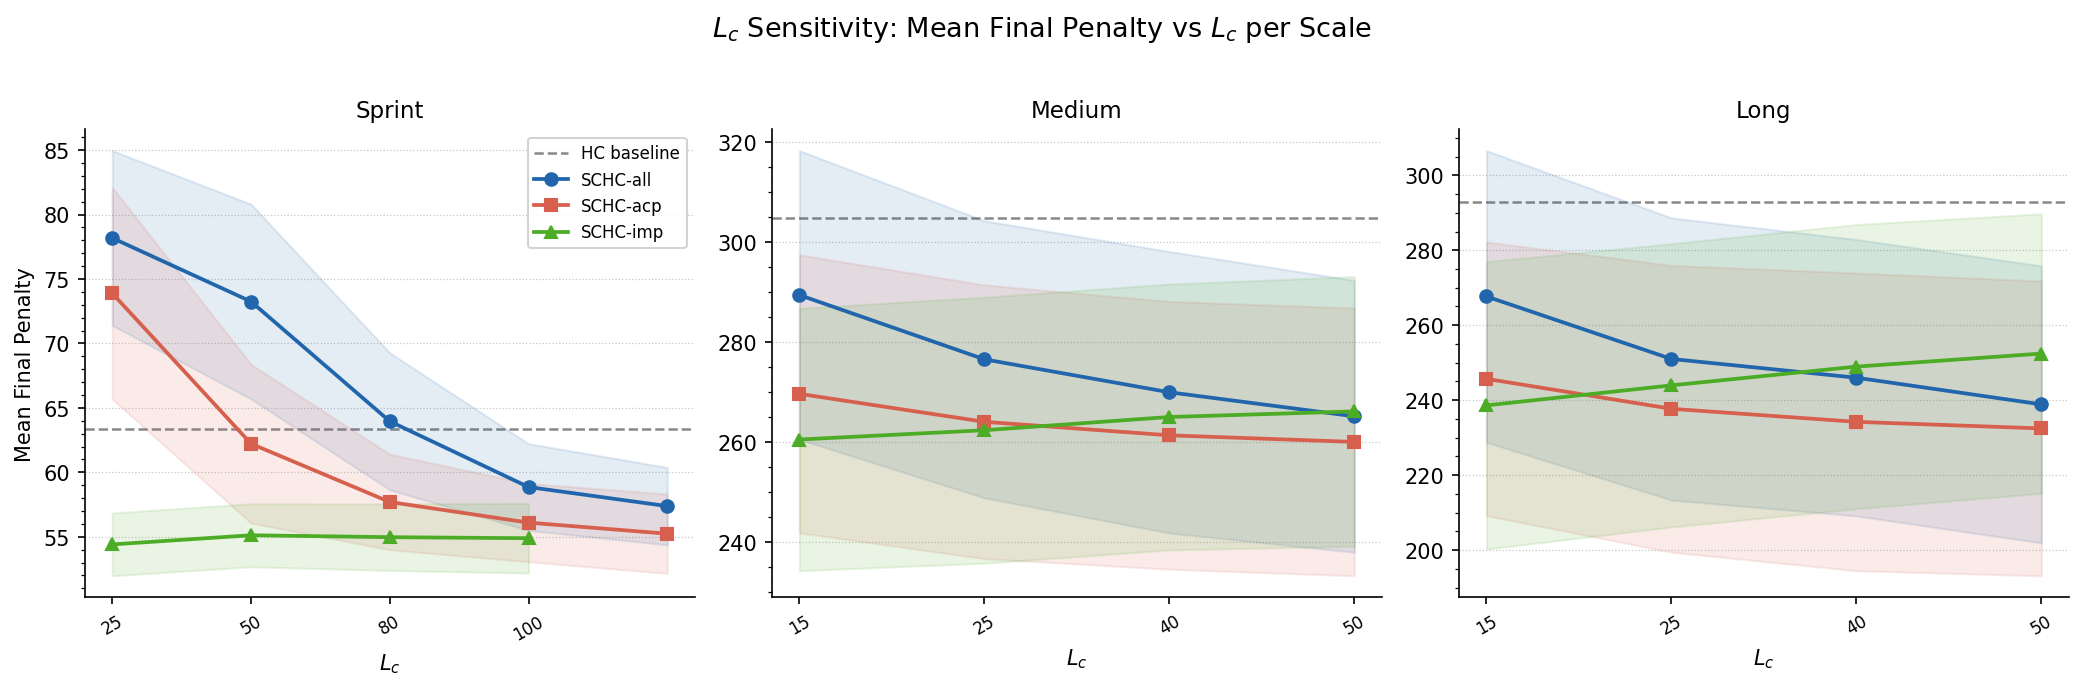
\includegraphics[width=\textwidth]{fig1_lc_sensitivity.png}
    \caption{Mean final penalty as a function of $L_c$ for SCHC-all,
    SCHC-acp, and SCHC-imp across Sprint, Medium, and Long scales.
    The shaded band indicates $\pm 1$ standard deviation. The dashed
    horizontal line marks the HC baseline mean. Note that SCHC-imp
    operates on a different $L_c$ scale to SCHC-all and SCHC-acp.}
    \label{fig:lc_sensitivity}
\end{figure}

\newpage
\subsection{Sprint Scale}
\label{sec:Sprint_sensitivity}

At Sprint scale, SCHC-all and SCHC-acp both exhibit a monotonically
decreasing penalty as $L_c$ increases from 100 to 1,500, with no
clear saturation evident within the tested range. SCHC-all improves
from a mean of 78.18 at $L_c = 100$ to 57.38 at $L_c = 1{,}500$.
SCHC-acp improves from 73.89 to 55.24 over the same range, and
achieves better solution quality than SCHC-all at every tested $L_c$
value. Both variants fall below the HC baseline of 63.40 from
$L_c = 500$ onwards.

SCHC-imp behaves markedly differently. Its mean penalty at $L_c = 25$
(54.41) is already lower than the best result achieved by SCHC-all or
SCHC-acp at their highest tested $L_c$ values. Performance is
essentially flat across the SCHC-imp range: increasing $L_c$ from 25
to 100 produces negligible change in mean penalty, remaining within
the interval $[54.41, 55.12]$. SCHC-imp achieves the best mean
penalty of all variants at Sprint scale, and does so at a
substantially smaller parameter value than either SCHC-all or
SCHC-acp require to approach competitive performance.

\subsection{Medium scale}
\label{sec:Medium_sensitivity}

At Medium scale, the pattern for SCHC-all and SCHC-acp is broadly
consistent with Sprint: both improve monotonically across the swept
$L_c$ range, with SCHC-all declining from 289.38 at $L_c = 500$ to
265.16 at $L_c = 2{,}500$, and SCHC-acp from 269.64 to 260.04.
SCHC-acp again dominates SCHC-all at every tested value. Neither
variant reaches a clear plateau within the sweep range, suggesting
that further improvement may be achievable at higher $L_c$ values,
albeit at proportionally greater computational cost.

For SCHC-imp, the sensitivity profile inverts relative to Sprint:
penalty now increases monotonically with $L_c$, rising from 260.52
at $L_c = 15$ to 266.14 at $L_c = 50$. The minimum penalty of
SCHC-imp (260.52) is within 0.5 penalty points of SCHC-acp's minimum
(260.04), but is achieved at $L_c = 15$ rather than $L_c = 2{,}500$.
This inversion of the SCHC-imp sensitivity curve from Sprint to
Medium scale is among the most notable findings of this study and is
discussed mechanistically in Chapter \ref{ch:discussion}.

\newpage
\subsection{Long scale}
\label{sec:Long_sensitivity}

At Long scale, SCHC-all and SCHC-acp continue to improve with
increasing $L_c$. SCHC-all declines from 267.68 at $L_c = 500$ to
238.88 at $L_c = 2{,}500$; SCHC-acp declines from 245.70 to 232.46.
SCHC-acp achieves the lowest mean penalty among all three variants
at this scale.

SCHC-imp again shows a monotonically increasing penalty with $L_c$,
from 238.62 at $L_c = 15$ to 252.44 at $L_c = 50$. The minimum
penalty of SCHC-imp (238.62) is nearly identical to that of SCHC-all
(238.88), representing a convergence of these two variants that
contrasts sharply with their relative performance at Sprint scale,
where SCHC-imp was the clear leader by a margin of approximately 3
penalty points.

\begin{table}[H]
\centering
\caption{Mean final penalty by $L_c$ for each algorithm and scale.
HC baseline means are shown for reference. Bold entries indicate
the optimal $L_c$ for each variant within each scale.}
\label{tab:lc_sweep}
\footnotesize
\setlength{\tabcolsep}{4pt}
\begin{tabular}{llrrrrr}
\toprule
Scale & Algorithm & \multicolumn{5}{c}{$L_c$ / Mean Penalty} \\
\cmidrule(lr){3-7}
 & & \multicolumn{1}{c}{Value 1} & \multicolumn{1}{c}{Value 2}
   & \multicolumn{1}{c}{Value 3} & \multicolumn{1}{c}{Value 4}
   & \multicolumn{1}{c}{Value 5} \\
\midrule
\multirow{4}{*}{Sprint}
  & HC       & \multicolumn{5}{c}{63.40 (baseline)} \\
  & SCHC-all & 100: 78.18 & 250: 73.25 & 500: 63.96 & 1000: 58.86 & \textbf{1500: 57.38} \\
  & SCHC-acp & 100: 73.89 & 250: 62.22 & 500: 57.70 & 1000: 56.10 & \textbf{1500: 55.24} \\
  & SCHC-imp & \textbf{25: 54.41} & 50: 55.12 & 80: 54.97 & 100: 54.89 & \\
\midrule
\multirow{4}{*}{Medium}
  & HC       & \multicolumn{5}{c}{304.86 (baseline)} \\
  & SCHC-all & 500: 289.38 & 1000: 276.54 & 1500: 269.96 & \textbf{2500: 265.16} & \\
  & SCHC-acp & 500: 269.64 & 1000: 264.06 & 1500: 261.36 & \textbf{2500: 260.04} & \\
  & SCHC-imp & \textbf{15: 260.52} & 25: 262.38 & 40: 265.02 & 50: 266.14 & \\
\midrule
\multirow{4}{*}{Long}
  & HC       & \multicolumn{5}{c}{292.88 (baseline)} \\
  & SCHC-all & 500: 267.68 & 1000: 251.00 & 1500: 246.00 & \textbf{2500: 238.88} & \\
  & SCHC-acp & 500: 245.70 & 1000: 237.70 & 1500: 234.22 & \textbf{2500: 232.46} & \\
  & SCHC-imp & \textbf{15: 238.62} & 25: 243.96 & 40: 248.96 & 50: 252.44 & \\
\bottomrule
\end{tabular}
\end{table}

\newpage
\section{Cross-Scale Performance at Optimal \texorpdfstring{$L_c$}{Lc}}
\label{sec:cross_scale}

Table \ref{tab:cross_scale} and Figure \ref{fig:cross_scale_bars}
summarise algorithm performance at the empirically optimal $L_c$ for
each variant and scale, including the improvement relative to the HC
baseline.

\begin{table}[H]
\centering
\caption{Algorithm performance at optimal $L_c$ per scale. All SCHC
variants are significantly better than HC at all scales ($p$ value $< 0.001$,
see Section \ref{sec:stats_tests}). The `vs HC' column reports the
mean penalty reduction relative to HC.}
\label{tab:cross_scale}
\begin{tabular}{llrrrr}
\toprule
Scale & Algorithm & Opt $L_c$ & Mean & Std & vs HC \\
\midrule
\multirow{4}{*}{Sprint}
  & HC        & --   & 63.40 & 4.83 & -- \\
  & SCHC-all  & 1500 & 57.38 & 3.01 & $-$6.02 ($-$9.5\%) \\
  & SCHC-acp  & 1500 & 55.24 & 3.08 & $-$8.16 ($-$12.9\%) \\
  & SCHC-imp  & 25   & 54.41 & 2.44 & $-$8.99 ($-$14.2\%) \\
\midrule
\multirow{4}{*}{Medium}
  & HC        & --   & 304.86 & 28.60 & -- \\
  & SCHC-all  & 2500 & 265.16 & 27.16 & $-$39.70 ($-$13.0\%) \\
  & SCHC-acp  & 2500 & 260.04 & 26.74 & $-$44.82 ($-$14.7\%) \\
  & SCHC-imp  & 15   & 260.52 & 26.20 & $-$44.34 ($-$14.5\%) \\
\midrule
\multirow{4}{*}{Long}
  & HC        & --   & 292.88 & 35.44 & -- \\
  & SCHC-all  & 2500 & 238.88 & 36.98 & $-$54.00 ($-$18.4\%) \\
  & SCHC-acp  & 2500 & 232.46 & 39.33 & $-$60.42 ($-$20.6\%) \\
  & SCHC-imp  & 15   & 238.62 & 38.35 & $-$54.26 ($-$18.5\%) \\
\bottomrule
\end{tabular}
\end{table}

\begin{figure}[H]
    \centering
    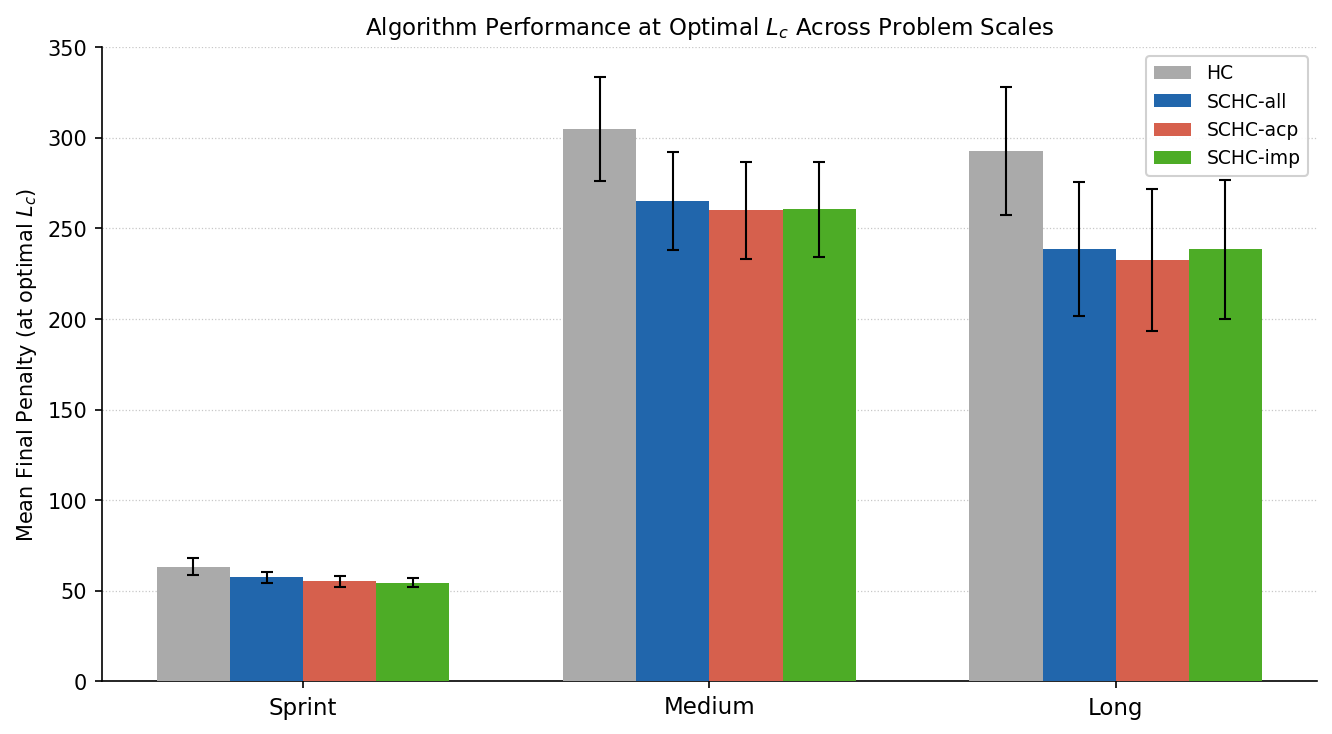
\includegraphics[width=0.88\textwidth]{fig2_cross_scale_bars.png}
    \caption{Mean final penalty at optimal $L_c$ for each algorithm
    across Sprint, Medium, and Long scales. Error bars represent
    $\pm 1$ standard deviation. All SCHC variants achieve
    substantially lower penalties than HC at all scales.}
    \label{fig:cross_scale_bars}
\end{figure}

Across all three scales, all SCHC variants reduce mean penalty
relative to HC by margins ranging from 6.0 to 60.4 penalty points.
At Sprint scale, SCHC-imp achieves the lowest mean penalty (54.41),
followed closely by SCHC-acp (55.24) and then SCHC-all (57.38). At
Medium scale, SCHC-acp and SCHC-imp are nearly identical in
performance (260.04 and 260.52 respectively), with both substantially
outperforming SCHC-all (265.16). At Long scale, SCHC-acp is the clear
leader (232.46), while SCHC-all and SCHC-imp converge to nearly
identical performance (238.88 and 238.62 respectively).

The trajectory of SCHC-imp relative to the other variants across
scales is particularly noteworthy: from best performer at Sprint
($-$14.2\% vs HC), through statistical equivalence with SCHC-acp at
Medium, to statistical equivalence with SCHC-all at Long. Figure
\ref{fig:variant_comparison} illustrates this convergence.

\begin{figure}[H]
    \centering
    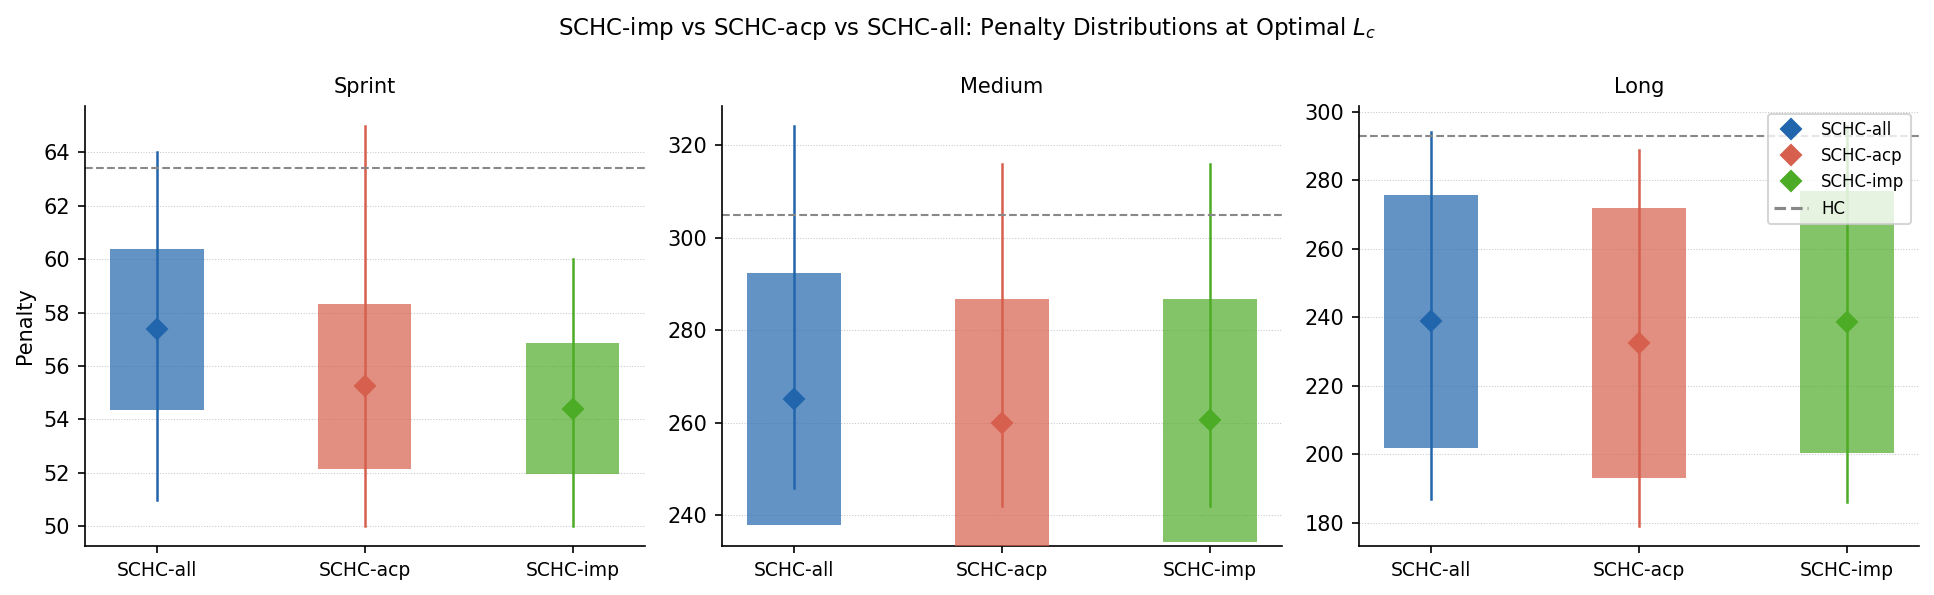
\includegraphics[width=\textwidth]{fig3_variant_comparison.png}
    \caption{Penalty distributions at optimal $L_c$ for each SCHC
    variant across scales. Diamonds mark the mean; bars span
    $\pm 1$ standard deviation; thin lines extend to the minimum and
    maximum observed values. The dashed line marks the HC baseline.
    Note the convergence of SCHC-imp and SCHC-all at Long scale.}
    \label{fig:variant_comparison}
\end{figure}

\section{Statistical Comparisons}
\label{sec:stats_results}
\label{sec:stats_tests}
 
Table~\ref{tab:per_instance} reports the mean final penalty for each
algorithm at optimal $L_c$, broken down by individual problem instance.
This per-instance view demonstrates that the aggregate performance patterns
reported in Table~\ref{tab:cross_scale} are consistent across all instances
within each scale tier and are not driven by any single outlying instance.
 
\begin{table}[H]
\centering
\caption{Mean final penalty (10 runs) at optimal $L_c$ per instance,
across all three problem scales. Optimal $L_c$ values: SCHC-all and
SCHC-acp at $L_c = 1{,}500$ (Sprint) and $L_c = 2{,}500$ (Medium,
Long); SCHC-imp at $L_c = 25$ (Sprint) and $L_c = 15$ (Medium, Long).}
\label{tab:per_instance}
\small
\begin{tabular}{llrrrr}
\toprule
Scale & Instance & HC & SCHC-all & SCHC-acp & SCHC-imp \\
\midrule
\multirow{10}{*}{Sprint}
  & Sprint\_01 & 63.3 & 58.3 & 55.0 & 54.6 \\
  & Sprint\_02 & 66.9 & 60.5 & 57.1 & 56.6 \\
  & Sprint\_03 & 60.7 & 54.3 & 51.3 & 50.9 \\
  & Sprint\_04 & 72.2 & 61.3 & 60.7 & 58.2 \\
  & Sprint\_05 & 62.0 & 57.6 & 55.8 & 55.0 \\
  & Sprint\_06 & 59.6 & 54.7 & 52.9 & 52.9 \\
  & Sprint\_07 & 63.8 & 58.7 & 56.7 & 56.0 \\
  & Sprint\_08 & 62.8 & 57.4 & 53.9 & 53.2 \\
  & Sprint\_09 & 64.0 & 57.5 & 56.8 & 55.6 \\
  & Sprint\_10 & 58.7 & 53.5 & 52.2 & 51.1 \\
\midrule
\multirow{5}{*}{Medium}
  & Medium\_01 & 291.8 & 253.3 & 249.4 & 250.4 \\
  & Medium\_02 & 295.1 & 253.6 & 246.9 & 247.4 \\
  & Medium\_03 & 284.1 & 250.1 & 244.7 & 245.2 \\
  & Medium\_04 & 295.3 & 250.4 & 246.5 & 247.5 \\
  & Medium\_05 & 358.0 & 318.4 & 312.7 & 312.1 \\
\midrule
\multirow{5}{*}{Long}
  & Long\_01 & 254.5 & 194.2 & 183.2 & 190.2 \\
  & Long\_02 & 288.7 & 218.3 & 208.2 & 217.4 \\
  & Long\_03 & 259.1 & 218.7 & 215.8 & 220.3 \\
  & Long\_04 & 337.2 & 290.0 & 286.5 & 291.9 \\
  & Long\_05 & 324.9 & 273.2 & 268.6 & 273.3 \\
\bottomrule
\end{tabular}
\end{table}

 
The ordering of SCHC-all $>$ SCHC-acp $\approx$ SCHC-imp in mean penalty
is consistent across every Sprint instance. At Medium scale, SCHC-acp and
SCHC-imp are within 1.0 penalty point of each other on all five instances,
while remaining clearly below SCHC-all. At Long scale, the pattern is less
uniform: SCHC-acp achieves the lowest mean penalty on instances Long\_01
through Long\_03, while SCHC-imp and SCHC-all converge on instances Long\_04
and Long\_05. Instance Medium\_05 and Long\_04 both return substantially
higher penalties than their scale counterparts across all algorithms,
reflecting the greater constraint complexity of those particular instances.
 
Table~\ref{tab:wilcoxon} reports the results of Wilcoxon signed-rank tests
for all pairwise comparisons at optimal $L_c$ per scale. All tests use
individual runs paired by instance and random seed, with $N = 100$
pairs at Sprint scale and $N = 50$ at Medium and Long scales. Bold $p$ values indicate statistical significance
at $\alpha = 0.05$.


\begin{table}[H]
\centering
\caption{Wilcoxon signed-rank test results for pairwise algorithm
comparisons at optimal $L_c$ per scale. Effect size
$r = |Z|/\sqrt{N}$, with $Z$ obtained from the two-sided $p$ value
through the normal approximation. Bold $p$ values indicate
statistical significance at $\alpha = 0.05$; non-bold entries are
not significant.}
\label{tab:wilcoxon}
\small
\begin{tabular}{llrrrrr}
\toprule
Scale & Comparison & $\Delta$ Mean & Statistic & $p$ value & Effect $r$ \\
\midrule
\multirow{6}{*}{Sprint}
  & SCHC-all vs HC       & $-$6.02 & 57.5  & \textbf{$<$ 0.001} & 0.840 \\
  & SCHC-acp vs HC       & $-$8.16 & 1.0   & \textbf{$<$ 0.001} & 0.869 \\
  & SCHC-imp vs HC       & $-$8.99 & 0.0   & \textbf{$<$ 0.001} & 0.865 \\
  & SCHC-acp vs SCHC-all & $-$2.14 & 453.0 & \textbf{$<$ 0.001} & 0.660 \\
  & SCHC-imp vs SCHC-all & $-$2.97 & 48.5  & \textbf{$<$ 0.001} & 0.827 \\
  & SCHC-imp vs SCHC-acp & $-$0.83 & 580.5 & \textbf{$<$ 0.001} & 0.380 \\
\midrule
\multirow{6}{*}{Medium}
  & SCHC-all vs HC       & $-$39.70 & 0.0  & \textbf{$<$ 0.001} & 0.870 \\
  & SCHC-acp vs HC       & $-$44.82 & 0.0  & \textbf{$<$ 0.001} & 0.871 \\
  & SCHC-imp vs HC       & $-$44.34 & 0.0  & \textbf{$<$ 0.001} & 0.870 \\
  & SCHC-acp vs SCHC-all & $-$5.12  & 38.0 & \textbf{$<$ 0.001} & 0.777 \\
  & SCHC-imp vs SCHC-all & $-$4.64  & 56.5 & \textbf{$<$ 0.001} & 0.761 \\
  & SCHC-imp vs SCHC-acp & $+$0.48  & 420.5 & $= 0.270$          & 0.156 \\
\midrule
\multirow{6}{*}{Long}
  & SCHC-all vs HC       & $-$54.00 & 0.0  & \textbf{$<$ 0.001} & 0.870 \\
  & SCHC-acp vs HC       & $-$60.42 & 0.0  & \textbf{$<$ 0.001} & 0.870 \\
  & SCHC-imp vs HC       & $-$54.26 & 0.0  & \textbf{$<$ 0.001} & 0.870 \\
  & SCHC-acp vs SCHC-all & $-$6.42  & 77.0 & \textbf{$<$ 0.001} & 0.742 \\
  & SCHC-imp vs SCHC-all & $-$0.26  & 531.0 & $= 0.917$          & 0.015 \\
  & SCHC-imp vs SCHC-acp & $+$6.16  & 59.0 & \textbf{$<$ 0.001} & 0.791 \\
\bottomrule
\end{tabular}
\end{table}


At Sprint scale, every pairwise comparison is statistically
significant at $p$ value $< 0.001$, including the comparison between
SCHC-imp and SCHC-acp ($p$ value $< 0.001$, $r = 0.380$). All effect sizes
relative to HC are large ($r > 0.84$). At Medium scale, the
comparison between SCHC-imp and SCHC-acp is not significant ($p =
0.270$, $r = 0.156$), indicating that the advantage of SCHC-imp
observed at Sprint scale has been eliminated. Both remain
significantly better than SCHC-all ($p$ value $< 0.001$). At Long scale,
the SCHC-imp versus SCHC-all comparison is not significant ($p =
0.917$, $r = 0.015$), confirming near-complete equivalence of these
two variants. SCHC-acp is significantly better than both SCHC-all
and SCHC-imp at Long scale ($p$ value $< 0.001$, $r > 0.74$).



\section{Comparison with Published Benchmark Results}
\label{sec:validation}

The penalty function used in this study was validated prior to
experimentation by evaluating best-known solutions published by
\citet{Toffolo2014} against the implemented evaluator. Across seven
instances spanning all three scales (Sprint01 to Sprint05, Medium01
and Long05), discrepancies ranged from 0 to 7 penalty points relative
to the published values, consistently in the direction of
under-penalisation. The mean absolute discrepancy was 1.6 percent of
the published penalty. Two instances from Sprint scale and one from
Medium scale returned exact agreement (discrepancy = 0). This pattern
is consistent with minor implementation differences in a small number
of soft constraint edge cases.

This validation measures the evaluator's error on published
solutions, which were not optimised against it. It does not bound
the error on the solutions found in this study, which were. As
Table~\ref{tab:hhsa_comparison} shows, the best result obtained here
lies below the published best-known solution on all ten Sprint and
Long instances compared, by between 1 and 27 penalty points. On
Sprint01, for example, the evaluator agrees exactly with the
published value of 56 for the best-known solution, yet the best
solution found in this study scores 53. Improving on the best
published results for a heavily studied benchmark with a
single-parameter local search is implausible. The more likely
explanation is that each algorithm, in minimising the penalty as
computed by this evaluator, was drawn towards solutions that contain
violations the evaluator fails to penalise. All algorithms in this
study were scored by the same evaluator, so the comparisons between
them are unaffected. Absolute penalty values, however, are optimistic
by an unknown margin and should not be compared with results
reported elsewhere. Rescoring the best solutions with the official
INRC-I validator would resolve the question and is left to future
work.

For context, Table \ref{tab:hhsa_comparison} sets the best results
achieved in this study alongside those reported by
\citet{Awadallah2015} for the Hybrid Harmony Search Algorithm (HHSA)
on the same INRC-I early instances, and alongside the best-known
solutions. For the reasons given above, and because the HHSA
experiments used different hardware and time budgets, these figures
are not directly comparable and no conclusion about relative
performance is drawn from them.

\begin{table}[H]
\centering
\caption{Comparison of best result (minimum penalty over all SCHC runs)
against HHSA reported results by \citet{Awadallah2015} on selected
INRC-I instances. Asterisked HHSA entries indicate runs that reached
the competition time limit. BKS denotes the current best-known
solution from \citet{Toffolo2014}.}
\label{tab:hhsa_comparison}
\small
\begin{tabular}{llrrr}
\toprule
Instance & This study (best) & HHSA $f_{\text{avg}}$ & BKS \\
\midrule
Sprint01 & 53 & 56.5 & 56 \\
Sprint02 & 55 & 58.5 & 58 \\
Sprint03 & 50 & 51.8 & 51 \\
Sprint04 & 57 & 60.1 & 59 \\
Sprint05 & 54 & 58.1 & 58 \\
\midrule
Long01 & 179 & 200.2$^*$ & 197 \\
Long02 & 202 & 228.7$^*$ & 226 \\
Long03 & 213 & 240.0$^*$ & 240 \\
Long04 & 283 & 305.1$^*$ & 303 \\
Long05 & 264 & 285.7$^*$ & 284 \\
\bottomrule
\end{tabular}
\end{table}

The apparent advantage of this study's results over both the HHSA
averages and the best-known solutions at Sprint and Long scale is
therefore attributed to the evaluator rather than to the algorithms.
At Medium scale, the best result in this study (242) is close to the
HHSA average of approximately 241--244, and the best result on
Medium01 (245) lies above its best-known value of 240.

%% ============================================================
\chapter{Discussion}
\label{ch:discussion}
%% ============================================================

This chapter interprets the experimental results presented in Chapter
\ref{ch:results} in terms of the underlying algorithmic behaviour of
the three SCHC variants, the properties of the INRC-I problem
landscape, and the broader implications for the application of
single-parameter metaheuristics to nurse rostering. Section
\ref{sec:disc_hc} discusses the consistent advantage of all SCHC
variants over HC. Section \ref{sec:disc_acp} addresses the
robustness of SCHC-acp across scales. Sections \ref{sec:disc_imp_lc}
and \ref{sec:disc_imp_degrade} provide a mechanistic account of
SCHC-imp's scale-invariant optimal $L_c$ and its performance
degradation at larger scales respectively. Section
\ref{sec:disc_theoretical_lc} revisits the theoretical $L_c$
recommendation in light of the empirical findings. Section
\ref{sec:limitations} addresses the limitations of the study.

\section{Superiority of SCHC over Hill Climbing}
\label{sec:disc_hc}

The most unambiguous finding of this study is that all three SCHC
variants significantly outperform the Hill Climbing baseline across
every scale and instance tested, with large effect sizes ($r > 0.84$,
$p$ value $< 0.001$ in all cases). This result confirms the core premise of
the SCHC framework: by holding the cost bound $B_c$ fixed for a
prescribed number of steps rather than updating it at every
iteration, the algorithm is able to accept non-improving moves
temporarily, thereby escaping local optima that trap pure HC. The
magnitude of the improvement is substantial: reductions of between
6.0 and 60.4 penalty points relative to HC, representing relative
improvements of 9.5 percent to 20.6 percent depending on scale and
variant.

This is consistent with the findings of \citet{Bykov2016} in the
examination timetabling domain, where all SCHC variants outperformed
HC on every benchmark instance. The result also aligns with the
broader literature on the NRP, where \citet{Awadallah2015, Hadwan2019} consistently found that
methods permitting acceptance of non-improving moves outperform
greedy hill climbing . The present
study extends this finding to the SCHC framework specifically, on the
INRC-I benchmark, and demonstrates that it holds robustly across
problem scales spanning a considerable range of instance complexity.

\section{Robustness of SCHC-acp Across Scales}
\label{sec:disc_acp}

SCHC-acp is the most consistently effective variant across all three
problem scales. At Sprint scale it is the second-best performer,
statistically inferior to SCHC-imp but superior to SCHC-all. At
Medium scale it is statistically equivalent to SCHC-imp and
significantly better than SCHC-all. At Long scale it is the outright
best performer, significantly superior to both SCHC-imp and SCHC-all.

The explanation for this robustness lies in the coupling between the
bound-update frequency and the acceptance rate of the search. Because
SCHC-acp increments its counter only on accepted moves, the effective
number of search iterations per bound update is implicitly regulated
by the problem landscape: when the search is in a productive region
and accepting moves frequently, the bound updates more rapidly; when
the search stagnates and fewer moves are accepted, the bound is held
for Longer, giving the algorithm more time to find an improving
direction. This self-regulating behaviour makes SCHC-acp
comparatively insensitive to the choice of $L_c$ relative to
SCHC-all, and also makes it more adaptive to the evolving difficulty
of the search as the algorithm approaches convergence.

SCHC-all, by contrast, increments its counter on every iteration
regardless of outcome. Its bound-update schedule is therefore
determined entirely by wall-clock iteration count, with no coupling
to the state of the search. This makes SCHC-all's behaviour more
predictable but also less adaptive, which may explain why it
consistently underperforms SCHC-acp at equivalent $L_c$ values.

\section{SCHC-imp: Scale-Invariant Optimal $L_c$ and the Improving Move Rate}
\label{sec:disc_imp_lc}

The most striking finding concerning SCHC-imp is that its empirically
optimal $L_c$ is not only small in absolute terms but is
approximately scale-invariant: the optimal value is $L_c = 25$ at
Sprint scale and $L_c = 15$ at Medium and Long scales, compared to
$L_c = 1{,}500$ and $L_c = 2{,}500$ for SCHC-all and SCHC-acp. This
is a marked departure from the behaviour reported by \citet{Bykov2016}
in the examination timetabling domain, where SCHC-imp's optimal $L_c$
was found to scale in a manner broadly comparable to the other
variants.

A mechanistic explanation is provided by the improving move rate
observed in this study. Across all Sprint runs at optimal $L_c$, improving moves account for
1.18 percent of total iterations for SCHC-imp, compared to 9.02
percent for SCHC-all and 5.70 percent for SCHC-acp. Because
SCHC-imp's counter increments only on improving moves, a nominal
$L_c$ of 25 corresponds to approximately 2,100 total iterations per
bound update at this rate (2,137 measured). This is broadly
comparable to the effective number of total iterations per bound
update for SCHC-all at $L_c = 1{,}500$ (1,515 measured). The apparent disparity in $L_c$ values between
variants is therefore partially an artefact of the differing
denominators of their counting rules: the improving move rate on the
NRP is so low that SCHC-imp's counter advances very slowly relative
to iteration count, making small $L_c$ values functionally equivalent
to much larger ones for the other variants.

This also explains why the optimal $L_c$ for SCHC-imp does not
increase substantially with problem scale, despite the problem
growing considerably in size and complexity. As the instance scale
increases, the improving move rate remains low throughout the search,
and the relationship between $L_c$ and effective bound-update
frequency remains governed by that rate. The consequence is that
SCHC-imp's operational regime on the NRP is structurally different
from that implied by the theoretical $L_c$ recommendation, which
assumes a much higher improving move rate than is empirically
observed.

\section{SCHC-imp Performance Degradation at Scale}
\label{sec:disc_imp_degrade}

The reversal of SCHC-imp's competitive standing from Sprint to Long
scale, from best performer to statistical equivalence with SCHC-all,
requires a separate explanation from the $L_c$ calibration argument
above.

At Sprint scale, SCHC-imp benefits from a favourable combination of
conditions: the problem is small enough that improving moves, though
rare, occur with sufficient frequency to update the cost bound
meaningfully before the search stagnates. The low improving move rate
is a constraint but not a fatal one, because the search space is
sufficiently navigable that the bound does update periodically and
the algorithm retains the ability to escape local optima.

As problem scale increases from Sprint to Medium to Long, the density
of the search landscape changes. Larger instances have more nurses,
more constraints, and more interacting soft constraint penalties. The
improving move rate, already low at Sprint scale, may decrease
further as the problem grows, reducing the frequency with which
SCHC-imp can update its cost bound. When the bound does not update,
SCHC-imp's acceptance criterion becomes static: it will accept any
move whose cost is no worse than the current solution, which is
equivalent to SCHC-all's behaviour under an infinitely large $L_c$.
In the extreme case where no improving moves are found for many
thousands of iterations, SCHC-imp effectively degenerates to a form
of random walk with a fixed acceptance bound, losing the adaptive
quality that distinguishes it from the simpler variants.

This hypothesis is consistent with the statistical results. At Long
scale, the SCHC-imp versus SCHC-all comparison yields $p$ value $= 0.917$
and $r = 0.015$, indicating near-complete equivalence. The
convergence of these two variants at Long scale, combined with the
mechanistic account above, suggests that SCHC-imp's effectiveness on
the NRP is contingent on the availability of a sufficient density of
improving moves to maintain meaningful bound updates throughout the
search. The NRP's constraint structure appears to produce a landscape
in which this condition is met at Sprint scale but progressively
eroded at larger scales.

It should be noted that this mechanistic account is necessarily
inferential. The improving move rate was directly measured only at
Sprint scale due to the availability of fine-grained iteration
statistics from the Sprint experiments. The claim that the improving
move rate decreases further at Medium and Long scales is a
hypothesis consistent with the observed performance pattern, but
direct measurement of bound update frequency across all scales and
variants would be required to confirm it. This represents a natural
extension of the present study.

\section{Empirical Optimal \texorpdfstring{$L_c$}{Lc} versus the Theoretical Recommendation}
\label{sec:disc_theoretical_lc}

\citet{Bykov2016} propose a theoretical optimal $L_c$ of
approximately $3.5 \times n$, where $n$ is the total number of
decision variables in the problem. For the INRC-I instances used in
this study, this yields values of approximately 1,000 at Sprint scale
and 2,000 to 3,000 at Medium and Long scales. The swept $L_c$ ranges
for SCHC-all and SCHC-acp were designed to cover this theoretical
range, and the empirical results are broadly consistent with the
recommendation: performance continues to improve up to $L_c = 1{,}500$
at Sprint and $L_c = 2{,}500$ at Medium and Long for both variants,
though without a clear plateau that would confirm saturation within
the tested range.

For SCHC-all and SCHC-acp, therefore, the theoretical recommendation
provides a useful and practically applicable guide for $L_c$
selection on the NRP, with the caveat that achieving the full benefit
requires HPC resources at Medium and Long scale, where convergence
times at $L_c = 2{,}500$ are measured in hours. This has implications
for the practical deployment of SCHC on real-world rostering
instances, where computation time is typically constrained.

For SCHC-imp, the theoretical recommendation is not applicable in
its standard form. The derivation of the $3.5 \times n$ heuristic
presumably assumes an improving move rate that is substantially
higher than the approximately 1 percent observed on the NRP.
Applying the standard recommendation to SCHC-imp would produce $L_c$
values that are computationally impractical and, as the empirical
data confirms, yield worse solutions than a much smaller $L_c$. A
revised calibration heuristic for SCHC-imp on problems with very
low improving move rates, perhaps expressed as a function of the
observed improving move rate rather than raw problem size, would be a
valuable contribution but is beyond the scope of this study.

\newpage
\section{Limitations and Future Work}
\label{sec:limitations}

Several limitations of this study warrant explicit acknowledgement.

\subsection{Single-Researcher Implementation}
\label{sec:disc_solo}

The algorithms and penalty function were implemented by a single
researcher without independent replication or external code review.
Whilst extensive steps were taken to validate the implementation,
including validation of the penalty function against best-known
solutions from \citet{Toffolo2014}, systematic testing of algorithm
behaviour against the specification of \citet{Bykov2016}, and
identification and correction of a defect in the initial variant
implementations in which the idle counter was not tracked uniformly
across variants (it is now reset by any accepted move for every
variant), the
possibility of residual implementation differences from the original
algorithm specification cannot be entirely excluded.

It is important to note, however, that the results are internally
coherent and mechanistically explicable. The behaviour of SCHC-imp,
in particular, follows a pattern that is well accounted for by the
measurable low improving move rate on the NRP, rather than
exhibiting the randomness or inconsistency that would typically be
associated with an implementation error. The statistical patterns
are robust, with large effect sizes and highly significant $p$ values
throughout. These considerations collectively support the integrity
of the reported results, but independent replication on the same
benchmark instances would further strengthen confidence in the
findings. The results are therefore best understood as a compelling
basis for a more rigorous follow-up study rather than as definitive
characterisations of SCHC behaviour on the NRP.

\subsection{Fidelity of the Penalty Function}
\label{sec:disc_evaluator}

As discussed in Section~\ref{sec:validation}, the best solutions
found in this study score below the published best-known solutions,
which indicates that the implemented evaluator misses some constraint
violations in the solutions the algorithms converge to. Relative
comparisons between algorithms, which share the evaluator, are
unaffected, but absolute penalties should not be compared with other
published results until the solutions have been rescored with the
official validator.

\subsection{Unit of Statistical Analysis}
\label{sec:disc_stats_unit}

The Wilcoxon tests treat each paired run as an independent
observation. Runs on the same instance share that instance's
structure, so the 100 Sprint pairs and 50 Medium and Long pairs are
not fully independent, and the reported $p$ values are likely to
overstate the strength of evidence relative to an analysis that
accounts for this grouping. The direction of the main effects is
consistent across individual instances (Table~\ref{tab:per_instance}),
which supports the conclusions, but a mixed-effects analysis with
instance as a grouping factor would give a more conservative test.

\subsection{Neighbourhood Structure}
\label{sec:disc_neighbourhood}

The study employed a single neighbourhood structure based on
reassignment and swap moves applied to individual nurse-day pairs.
The quality of solutions achievable by any local search method is
bounded by the connectivity of the neighbourhood: if the optimal
solution is not reachable from the starting solution by a sequence
of single-step moves, no local search algorithm can find it. The
choice of neighbourhood was not systematically optimised, and it is
possible that alternative or compound move operators would alter the
relative performance of the SCHC variants. This is a standard
limitation of local search studies and is noted here for
completeness.

\subsection{Further Investigation of SCHC-imp on the NRP}
\label{sec:disc_imp_future}

The behaviour of SCHC-imp on the NRP, and in particular its
performance degradation from Sprint to Long scale, was characterised
here at the level of summary statistics and aggregate improving move
rates. A more complete investigation would include direct measurement
of bound update frequency across all scales and variants, trajectory
analysis of the cost bound evolution over the course of individual
runs, and a systematic comparison of the improving move rate as a
function of instance scale and constraint density. Due to the time
constraints of this project, such analysis was not conducted, though
the experimental infrastructure developed here would support it with
modest additional effort. The unusual and theoretically interesting
behaviour of SCHC-imp on this problem class warrants dedicated
investigation in future work.

\subsection{Comparison with State-of-the-Art Methods}
\label{sec:disc_sota}

This study does not include a comprehensive comparison with
state-of-the-art methods on the INRC-I benchmark. The comparison
presented in Section \ref{sec:validation} is limited to the HHSA
of \citet{Awadallah2015} due to the availability of instance-level
results in that paper and the use of a compatible evaluation
framework. Methods achieving stronger results on the INRC-I
benchmark, including the competition winner, \citet{Valouxis2012},
and subsequent improvements, employ substantially more complex
hybrid architectures that are not directly comparable to the
single-parameter local search approach studied here. The goal of
this study is not to establish state-of-the-art performance but to
characterise the behaviour of a simple, interpretable metaheuristic
on a practically important problem class, and to assess whether its
properties in the examination timetabling domain transfer to the
nurse rostering context.

%% ============================================================
\chapter{Conclusion}
\label{ch:conclusion}
%% ============================================================

This dissertation set out to investigate whether the Step Counting
Hill Climbing Algorithm, previously evaluated exclusively in the
examination timetabling domain, transfers effectively to the Nurse
Rostering Problem, and to characterise how its sole free parameter,
the step counter limit $L_c$, should be calibrated as a function of
problem scale in this new domain. The study evaluated all three SCHC
variants against a Hill Climbing baseline across 20 problem instances
drawn from the INRC-I benchmark, spanning Sprint, Medium,
and Long scales, using systematic $L_c$ sweeps executed on
the Cardiff Falcon HPC cluster.

\section{Summary of Findings}
\label{sec:conc_summary}

The primary finding is unambiguous: all three SCHC variants
significantly outperform Hill Climbing at every problem scale tested,
with penalty reductions of between 9.5 and 20.6 percent and
consistently large effect sizes. This confirms that the core SCHC
mechanism, holding the cost bound fixed for a prescribed number of
steps to permit temporary acceptance of non-improving moves,
transfers successfully from examination timetabling to the nurse
rostering problem and delivers meaningful improvements over the
greedy baseline.

Beyond this primary result, the study yields three findings of
specific interest. First, SCHC-acp is the most robust variant across
scales, achieving the best performance at Long scale and statistical
equivalence with the leading variant at Medium scale. Its
acceptance-coupled counting mechanism appears to confer an adaptive
quality that is particularly well-suited to the evolving difficulty
of the NRP search landscape at larger problem sizes.

Second, SCHC-imp exhibits a scale-invariant optimal $L_c$ of 15 to
25, which is an order of magnitude smaller than the optimal values
observed for SCHC-all and SCHC-acp. This is explained by the
exceptionally low improving move rate on the NRP, approximately 1
percent of total iterations, which causes SCHC-imp's counter to
advance very slowly relative to total iteration count. As a
consequence, the standard theoretical $L_c$ recommendation of
$3.5 \times n$ is not applicable to SCHC-imp on this problem class
without revision.

Third, and most theoretically interesting, SCHC-imp degrades from
the best-performing variant at Sprint scale to statistical
equivalence with SCHC-all at Long scale. This convergence is
consistent with a progressive reduction in improving move
availability as problem complexity increases, which increasingly
prevents SCHC-imp from updating its cost bound and erodes the
behavioural distinction between this variant and the simpler
SCHC-all. This finding suggests that the effectiveness of SCHC-imp
is contingent on problem geometry in a way that does not apply to
SCHC-acp, and that SCHC-acp should be preferred for applications
where problem scale is large or unknown.

\section{Contributions}
\label{sec:conc_contributions}

This study makes three contributions to the existing literature.
It provides the first systematic evaluation of the SCHC algorithm
\citet{Bykov2016} on the INRC-I nurse rostering benchmark,
establishing a performance baseline for all three variants across
three problem scales. It identifies and provides a mechanistic
account of a previously unreported sensitivity of SCHC-imp to
problem geometry, specifically to the improving move rate of the
search landscape, which has implications for how the variant should
be applied to problems outside its original evaluation domain.
Finally, it shows that a single-parameter, schedule-free local search
algorithm delivers large and consistent improvements over Hill
Climbing on this benchmark, at modest computational cost relative to
more complex hybrid methods. Whether its absolute solution quality
is competitive with those methods remains to be established with the
official evaluator (Section~\ref{sec:disc_evaluator}).

\section{Future Work}
\label{sec:conc_future}

The most immediate extension of this work would be a direct
measurement of bound update frequency and improving move rate across
all three scales and variants, to test empirically the mechanistic
hypotheses advanced in Chapter \ref{ch:discussion}. A more thorough
characterisation of SCHC-imp's behaviour on the NRP, including
trajectory analysis of the cost bound and improving move rate over
the course of individual runs, would either confirm the proposed
explanation or reveal alternative dynamics that warrant further
investigation. Independent replication of the experimental results,
using a separately implemented codebase evaluated against the same
benchmark instances, would additionally strengthen confidence in the
reported findings.

At a broader level, it would be of interest to evaluate SCHC on
nurse rostering instances drawn from other benchmark datasets and
real hospital settings, to determine whether the parameter
sensitivities observed on the INRC-I early instances generalise to
other problem formulations. The question of whether a revised $L_c$
calibration heuristic for SCHC-imp, expressed as a function of the
empirically observed improving move rate rather than raw problem
size, could recover competitive performance at larger scales is also
a natural direction for future work.

\newpage
\section{Closing Remarks}
\label{sec:conc_closing}

The Step Counting Hill Climbing Algorithm is a genuinely simple
method: a single loop, a single parameter, and an acceptance rule
that can be stated in one line. The results of this study demonstrate
that this simplicity does not preclude strong performance on a
practically important and computationally challenging scheduling
problem. The more nuanced finding, that the three variants of SCHC
respond to the NRP's problem structure in meaningfully different
ways, and that these differences are scale-dependent in ways not
previously documented, suggests that the algorithm's apparent
simplicity conceals a richer set of behaviours than has been
characterised to date. Understanding those behaviours more fully
remains an open and worthwhile problem.

%% ============================================================
\appendix
\chapter{Revisions in this Edition}
\label{app:revisions}

The following changes were made to the version submitted in May
2026. In each case the text was corrected to agree with the final
results and code.

\begin{enumerate}
\item \textbf{Penalty validation (Section~\ref{sec:validation}).}
The validation was carried out on seven instances, not six. The
mean absolute discrepancy is now stated exactly (1.6 percent).
\item \textbf{Table~\ref{tab:lc_sweep}.} The $L_c = 1000$ results for
SCHC-all and SCHC-acp at Sprint scale, omitted from the submitted
version, have been added.
\item \textbf{Statistical method (Chapter~\ref{ch:introduction},
Section~\ref{sec:stats}, Section~\ref{sec:stats_results} and
Table~\ref{tab:wilcoxon}).} The submitted version stated that the Wilcoxon tests
were applied to per-instance means ($n = 10$ and $n = 5$) and that
$r$ was the matched-pairs rank-biserial correlation. The analysis
actually applied the tests to individual runs paired by instance and
seed ($N = 100$ and $N = 50$) and computed $r = |Z|/\sqrt{N}$. The
reported statistics were correct; their description has been
corrected. With $n = 5$, a two-sided Wilcoxon test cannot reach
$p < 0.05$, so the original description was also inconsistent with
the reported $p$ values.
\item \textbf{Table~\ref{tab:hhsa_comparison}.} Five best-result
values (Sprint01, Long02 to Long05) did not match the final results
and have been corrected. The Long04 and Long05 values in the
submitted version were lower than any result in the final data and
most likely came from runs of the pre-correction code that were
excluded from the final analysis.
\item \textbf{Interpretation of the comparison with published results
(Section~\ref{sec:validation}, Section~\ref{sec:disc_evaluator},
Section~\ref{sec:conc_contributions}).} The corrected best results
lie below the best-known solutions on every Sprint and Long instance
compared, which indicates that the evaluator under-penalises the
solutions found in this study. The claims that SCHC is competitive
with or better than HHSA have been withdrawn, and the third
contribution has been restated accordingly.
\item \textbf{Description of the corrected implementation defect
(Section~\ref{sec:disc_solo}).} The submitted version described the
idle-counter correction in reverse. The final implementation resets
the idle counter on any accepted move for every variant.
\item \textbf{Improving move rates (Section~\ref{sec:disc_imp_lc}).}
The rates quoted for Sprint scale (1.06, 9.35 and 5.92 percent) did
not match the final runs and have been replaced with the values
measured across all Sprint runs at optimal $L_c$ (1.18, 9.02 and 5.70
percent), together with the measured number of iterations per bound
update.
\item \textbf{Unit of statistical analysis.} A limitation on the
independence of runs within an instance has been added
(Section~\ref{sec:disc_stats_unit}).
\item \textbf{Bibliography.} The DOI of \citet{Bykov2016} has been
corrected.
\item The signature images on the declarations page have been
omitted from this public edition.
\end{enumerate}

%% ============================================================
\bibliography{references}

\end{document}